\section{Background}
\label{sec:Background}

\subsection{Introduction}

High Performance Computing (HPC) initiatives over the past decade have 
fostered the development of extremely successful scalable analysis tools ---
such as ParaView, VisIt, and Ensight --- that make it possible to visualize 
and explore very large datasets.  This success provides a foundation for 
the analysis we will do at Exascale, but the core disruptions caused by
the push to Exasacle --- disruptions that will be experienced by the entire
software stack, as well as the science codes --- will force us to fundamentally
change how we do \vda in the years ahead.

Current visualization and data analysis is largely done as an
\keyterm{offline post-processing} step, in which interactive visualization
tools read in data saved to disk, and an analyst sitting at a desk
interacts with that data in real time.  This method uses the disk as a
communication mechanism between the science code and the \vda application,
so the code and interactive analysis are functionally decoupled.  There are
some efforts aimed at changing this workflow, but it remains the standard
way that people interact with their data.

At extreme scale, this offline workflow will break down due to 
the mismatch
between the rate at which we can create large data, and the rate at
which that data can be moved to persistent storage.  In fact, this
data movement will be so costly in terms of energy that it will be
cost prohibitive to move results from memory to persistent storage 
\fix{citation needed}.
Because of this, extreme scale computing will have integrated \vda as a
method of determining what data are of interest and therefore worth
committing to persistent storage.

This data can be visualized interactively, analyzed,
sent to a data-centric computation, or written to persistent
storage.  Depending upon the needs of the end-user analysis, one or
more of these data collaboration steps may be requested.  The design
of the computation system --- from compute architecture through system
software and persistent storage model --- will be determined by the
needs of the analysis being performed at the end of the compute
cycle.  This system level co-design must take into account the
constraints of the compute resources (power, time, and cost), as
well as the requirements of the science and exploration to be done
at the conclusion of the scientific simulation.

\subsection{Current Post-Processing Pipelines}

The current prevalent practice of computational-based scientific analysis
is a progression of relatively independent steps.  First is a problem
setup, which involves defingin initial and boundary conditions,
determining materials and their properties, and creating a mesh or
establishing a meshing procedure.  Based on this problem setup, a
simulation is next run.  During the progression of the simulation, results
files are periodically recorded to disk storage.  This results data are
typically the geometry of physical entities being simulated (often but not
always a mesh of finite elements) with field values of physical properties
given for the topological units of the geometry.  Because of limitations
with disk storage bandwidth and capacity, results data seldom capture all
computed interactions but rather capture data at some periodicity specified
by the analyst.  At some time later, a \vda job reads this data back from
disk and presents an interactive analysis session with a user.

This ``offline'' post-processing \vda offers many advantages that make it
the easiest way to perform visualization.  First, because the simulation
and visualization are run in completely different jobs and nominally at
different times, the \vda requires no additional resource overhead on the
simulation (other than the requisite storage of results to disk).  Second,
it makes the interface between simulation and visualization simple.  The
visualization needs only to understand the format used when the simulation
writes the data to disk.  Third, it makes scheduling and performing the
visualization, particularly when done by a human, much easier.  The
visualization job can be scheduled completely independently of the
simulation and at a time most convenient to the user.  Fourth, the results
data are placed in persistent storage, so any analysis not performed
immediately can be done at a later time if they are later deemed necessary.
Thus, when it is feasible, offline post-processing is a convenient and
effective mechanism for \vda.

\subsection{Extreme-scale Analysis: New Challenges}
\label{sec:NewChallenges}

Why is science at Extreme Scale so different from current practice?  Can't
we continue using the successfully deployed applications for this new
scale, if, like science codes, we adapt to the challenges of the new
architectures?\footnote{Adapting \vda codes to new exascale architectures
  is a mostly independent research challenge being met by other research
  projects\lcite{PISTON,Moreland2011:LDAV,EAVL,Sewell2012}.}

The answer is, simply, no.  A major challenge moving from current
architectures to extreme architectures and extreme scales is that the rate
of computation far outstrips the rate of I/O for a large system.  At some
point the relative bandwidth of the storage system is insufficient to make
the capturing of sufficient results data practical, and we believe such a
situation will occur at the exascale.

\begin{figure}[htb]
  \centering
  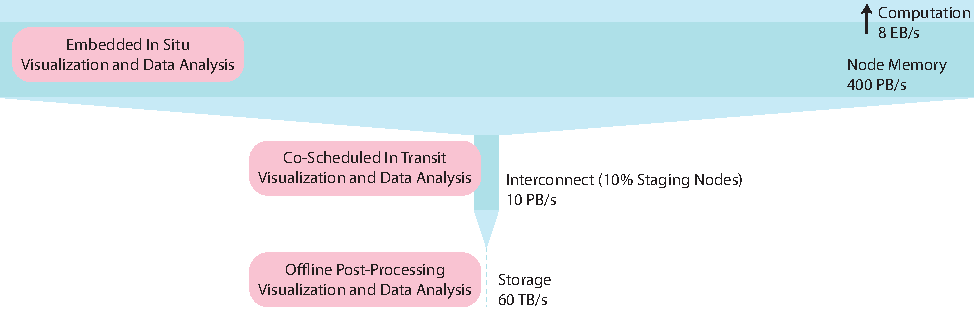
\includegraphics{figures/IOBandwidths}
  \caption[Relative bandwidth of exascale system components.]{Visual
    depiction of the relative bandwidth of exascale system components based
    on predictions of exascale
    machines\lcite{ScientificDiscoveryExascale2011,ExascaleArchitecturesReport}.}
  \label{fig:IOBandwidths}
\end{figure}

Figure~\ref{fig:IOBandwidths} provides a Minard plot depicting the
bandwidths of different I/O components by the proportional width of their
respective blue bars.  (See Tufte\scite{Tufte2001} for a longer description
of Minard plots and their merits.)  Not shown on this plot is the rate at
which data can be computed.  At $10^{18}$ double precision floating point
operations per second, the exascale computer on aggregate will produce 8~EB
per second.  On this plot that would be over 10 feet across.  The aggregate
bandwidth of the local memory --- that is, the speed at which data can be
pulled from memory to a local process summed over the entire machine --- is
400~PB/s.  This is as fast as we can reasonably expect to access data on
the system, but it is only available in the same job space as the running
simulation.  If we were to offload that data to another job, say a staging
job running on a generous allocation of 10\% of the overall nodes, then we
could stream the data to this job at 10~PB/s, which is pretty fast but only
2.5\% the local access rate.  Furthermore, one must worry about the limited
memory available on the staging nodes.  To move the data entirely to disk
storage, the bandwidth drops way down to 60~TB/s.  This is only 0.015\% the
rate at which data can be written to local memory and only 0.00075\% the
rate at which data can be computed.  So, only an extremely small fraction
of data can ever hope to be captured on disk.

Because there is such a disparity between computation rate and storage
bandwidth, \keyterm{\insitu visualization}, the visualization of data while
still present in the working memory of a simulation and before being
transferred to disk storage, features predominately in plans for near and
far term
\vda\lcite{ScientificDiscoveryExascale2011,VisualizationKnowledgeDiscovery2007,Childs2007,Moreland2012:Ultravis}.
An important consequence is the system wide implications resulting from the
solution to this problem, which include scientific domain specific analysis
techniques, \insitu framework development, and complexity impacts in
post-processing.

\fix{Dave originally had text arguing that another reason that data could
  not be saved to disk was the power cost.  However, I think the power cost
  is reflected in the bandwidth and capacity of the system.  Unless there
  is a further limitation of the system due to power, such as the peak
  bandwidth cannot be maintained due to power restrictions and will quickly
  be throttled back, or that there will be a measured cost added to
  projects to save more data, then I don't see the point of adding the
  extra detail.  I don't recall ever seeing any such predictions.}

\begin{figure}
  \centering
  \subfloat
      [Traditional offline post-processing \vda.]
      {
        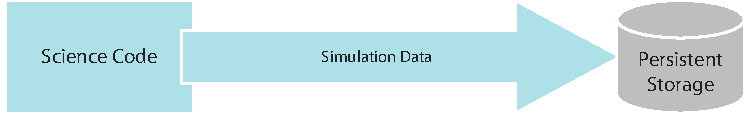
\includegraphics{figures/WorkflowsOffline}
        \label{fig:Workflows:Offline}
      } \\
  \subfloat
      [Embedded \insitu \vda (VDA).]
      {
        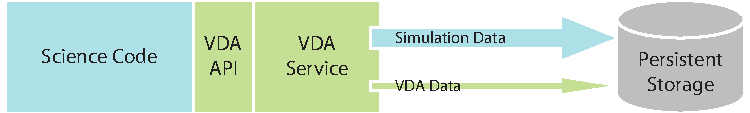
\includegraphics{figures/WorkflowsInSitu}
        \label{fig:Workflows:InSitu}
      } \\
  \subfloat
      [Service-oriented \intransit \vda (VDA).]
      {
        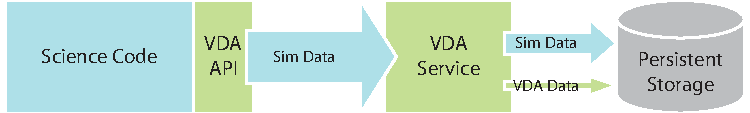
\includegraphics{figures/WorkflowsInTransit}
        \label{fig:Workflows:InTransit}
      }
  \caption[Visualization and data analysis workflows.]{Traditional and
    emerging workflow diagrams showing the flow of information from
    simulation to persistent storage.  In all cases data will later be
    retrieved from storage and further analyzed.}
  \label{fig:Workflows}
\end{figure}

Figure~\ref{fig:Workflows} shows simplified diagrams showing the flow of
information from simulation to persistent storage in a typical modeling and
simulation workflow.  Typical \vda occurs as an offline post-processing
step, after the simulation has written results directly to persistent
storage (Figure~\ref{fig:Workflows:Offline}).  Often, these results are in
a code-specific format, and are formatted as ``restart'' files ---
optimized for reading back into an instance of the science code, and not
optimized for post processing analysis by \vda tools.

Extreme computation size and extreme architectures force data flows like
those in Figures \ref{fig:Workflows:InSitu} and
\ref{fig:Workflows:InTransit} in which \vda is performed on the simulation
results before they are written to persistent storage.  In
Figure~\ref{fig:Workflows:InSitu}, data are handed directly to an
\keyterm{embedded \insitu} \vda library coupled with the running code,
enabling analysis, visualization and data reduction under the control of
the science code --- at the cost of sharing runtime resources with the \vda
execution.  In Figure~\ref{fig:Workflows:InTransit}, data are transferred
to an \keyterm{\intransit} \vda process separate from the running code.
This decouples the data computation and \vda processes, which affords many
advantages but at the cost of system complexity.  Both approaches must be
provided for extreme scale analysis, so that the codes, system designers,
and science customers can design a computation and analysis workflow suited
to the specific needs of the science, analysis, and decision process being
supported.

\subsection{Contributions}

To facilitate the transition to these new workflows, our group is
developing supporting technologies to help implement the tighter coupling
between simulation and \vda.  To this end we are contributing to two key
enabling projects: Catalyst and Nessie.

\keyterm{Catalyst} is an \insitu library that provides a simplified
interface to \vda through direct function calls.  The primary intention is
to provide a \vda service to simulation codes as demonstrated in the
workflow of Figure~\ref{fig:Workflows:InSitu}.  Catalyst is described in
more detail in Section~\ref{sec:Catalyst}.

\keyterm{Nessie} is an I/O service that provides remote-procedure call
abstractions and one-sided data-message passing.  Nessie makes
communication between parallel jobs more simple and efficient, and we use
it to facilitate the transfer of simulation data from simulation to \vda
service in the \intransit workflow of Figure~\ref{fig:Workflows:InTransit}.
Nessie is described in more detail in Section~\ref{sec:Nessie}.

With these tools we can implement the multiple workflows of
Figure~\ref{fig:Workflows} and compare their relative performance.  For
this comparison, we implement a use case, described in
Section~\ref{sec:UseCase}, which is representative of some real-world
problems being addressed by our users at Sandia National Laboratories.  The
results of these comparisons are given in Section~\ref{sec:Results}.
